\documentclass{article}
\usepackage[utf8]{inputenc}
\usepackage[russian]{babel}
\usepackage[inline]{asymptote}
\usepackage{amsmath,amssymb, amsfonts,amssymb,amsthm,mathtools}
\usepackage[urlcolor=blue]{hyperref}
\usepackage{natbib}
\usepackage{graphicx}
\usepackage{mathbbol}

\newtheorem{theorem}{Теорема}
\newtheorem{lemma}[theorem]{Лемма}
\theoremstyle{definition}
\newtheorem{definition}{Определение}

\DeclareMathOperator{\ME}{\mathbb{E}}
\DeclareMathOperator{\D}{\mathbb{D}}
\DeclareMathOperator{\prob}{\mathbb{P}}


\begin{document}
\title{\underline{\textbf{Теормин по ДГМС}}}
\author{Иван Кобзев}
\date{январь 2020}

\maketitle
\newpage
\textit{Забившим на ДГМС первой парой во вторник посвящается}
\newpage
Этот документ представляет собой теормин так, как я его понимаю. Естественно, что вполне возможны как неверное понимание, так и опечатки (почти наверное). Все замечания и исправления приветствуются. Материал был взят из чужого конспекта на диске (естетсвенно, я тоже не ходил), ссылка в центре страницы.\newline
\begin{asy}[width=\the\linewidth,inline=true]
pair z0=(-2,0);
pair z1=(0,0);
pair z2=(2,0);
pair zf0=(-1, -2);
pair zf1=(0, -2);
pair zf2=(1, -2);

draw(z0--zf0,red,Arrow,PenMargins);
draw(z1--zf1,orange,Arrow,PenMargins);
draw(z2--zf2,yellow,Arrow,PenMargins);
\end{asy}
\vspace{10mm}
\begin{center}
\href{https://yadi.sk/d/d-ti\_TZi3Mh3Ri/7\%20sem/\%D0\%94\%D0\%93\%D0\%9C\%D0\%A1}{Ссылка на конспект 2018 года}
\end{center}
\vspace{10mm}
\begin{asy}[width=\the\linewidth,inline=true]
pair z0=(2,0);
pair z1=(0,0);
pair z2=(-2,0);
pair zf0=(1, 2);
pair zf1=(0, 2);
pair zf2=(-1, 2);

draw(z0--zf0,green,Arrow,PenMargins);
draw(z1--zf1,blue,Arrow,PenMargins);
draw(z2--zf2,lightblue,Arrow,PenMargins);
\end{asy}
\newpage
\tableofcontents
\newpage

\section{Элементы теории риска}
Сама теория вероятностей зарождалась применительно к играм, так что довольно естественно начать обсуждение именно с игр. Предположим, есть некоторая игра, за участие в которой берут взнос, а в самой игре есть элемент случайности, от которого зависит выигрыш игрока. Нас будет интересовать простой вопрос: стоит ли принимать участие в игре? Первым приходящим на ум инструментом, который будет давать ответ на этот вопрос, служит матожидание. Ну, в самом деле, если посчитать, сколько в среднем мы выиграем, а потом сравнить это число со взносом за игру, то принимать участие стоит лишь тогда, когда средний выигрыш будет больше или, хотя бы, не меньше, чем взнос. Однако подобный подход работает не всегда с точки зрения жизненной логики, поэтому мы введём понятие функции полезности, с помощью которой получается более гибко описывать подобные ситуации.

Везде далее маленькими буквами $x, y, z, \ldots$ будем обозначать доходы или потери, а большими $X, Y, Z, \ldots$ -- случайные величины, соответствующие случайным же доходам или потерям игрока. 

Очевидно, что проще всего ввести предпочтение на множестве вещественных чисел естественным образом: $x \preceq y \Longleftrightarrow x \le y$, то есть предпочтительней тот доход, который численно больше (если же говорим о потерях, то в правой части знак естественно заменить на противоположный).

Договоримся рассматривать даже неслучайные доходы как случайные величины, только вырожденные (принимающие своё значение с вероятностью $1$). Тем самым вопрос становится чуть более глобальным: как по паре случайных величин ввести отношение предпочтения?

На этот вопрос есть два ответа, сразу приходящих на ум:
\begin{enumerate}
    \item $X \preceq Y \Longleftrightarrow X(\omega) \le Y(\omega), \forall \omega$ (редко, потому что слишком сильное условие)
    \item Как было уже сказано выше, матожидание, то есть $X \preceq Y \Longleftrightarrow \mathbb{E}X \le \mathbb{E}Y$.
\end{enumerate}
Почему же плох второй подход? Есть два примера:
\begin{enumerate}
    \item Рассмотрим две игры, в первой из которых (отвечающей с.в. $X$) вы с вероятностью $1$ выигрываете $500000\$$, а во второй (отвечающей с.в. $Y$) с вероятностью $0.1$ выигрываете $2500000\$$, с вероятностью $0.6$ выигрываете те же $500000$, но ещё есть вероятность $0.3$ потерять всё и уйти с пустыми руками. Естественно предпочесть первую игру второй, однако же подсчёт матожиданий показывает, что $\mathbb{E}Y > \mathbb{E}X$.
    \item Вторая игра известна как \textit{петербургский парадокс}. Пусть, играя в неё, мы выигрываем $2^k\$$ с вероятностью $\frac{1}{2^k}$. Матожидание игры равно $+\infty$, что значит, что в неё стоит играть при любом взносе. Однако же понятно, что с точки зрения жизненной логики никто не сядет играть в такую игру за большой взнос.
\end{enumerate}

Поэтому предлагается как-то изменить подход к введению отношения предпочтения, что приводит нас к 
\begin{definition}
Пусть на множестве случайных величин задано отношение предпочтения. Будем говорить, что на этом множестве задана \textit{функция полезности $u(x)$}, согласованная с этим отношением предпочтения, если 
$$X \preceq Y \longrightarrow \mathbb{E}u(X) \le \mathbb{E}u(Y)$$ $$X \prec Y \longrightarrow \mathbb{E}u(X) < \mathbb{E}u(Y)$$ $$X \sim Y \longrightarrow \mathbb{E}u(X) = \mathbb{E}u(Y)$$
\end{definition}
Тогда вопрос о том, до какого взноса стоит играть, имеет однозначный ответ и напрямую зависит от функции полезности, выбранной игроком. Например, в петербургском парадоксе достаточно взять $u(x) = \log(x)$, чтобы сразу получить точное верхнее значение взноса, равное $4\$$. Тем самым, функция полезности, которую для себя принял игрок, является неким показателем его отношения к риску (если в петербургском парадоксе взять $u(x) = x$, то мы отбитые на всю голову и готовы играть при любом взносе, если же $u(x) = \log(x)$, то допустимый для нас взнос уже не больше $4\$$).

Дальше идут теоремы о некоторых естественных свойствах функции полезности. 
\begin{theorem}
Если отношение предпочтение берётся на основании функции полезности $u(x)$, то $\forall a > 0, b \in \mathbb{R}$ функция $au(x) + b$ задаст то же самое отношение предпочтения.
\end{theorem}
\begin{theorem}
Для естественным образом введённого отношения предпочтения на неслучайных доходах (лучше тот доход, который больше), функция полезности не убывает, то есть для дифференцируемой функции полезности естественно условие $u'(x) \ge 0$.
\end{theorem}
Третью теорему не вижу смысла писать, по сути она говорит, что по известному дифференциалу мы можем определить саму функцию полезности.

Однако и функция полезности не является идеальным инструментом по той простой причине, что она может не существовать. Для примера доказываем сначала теорему. Если не совсем понятно, что в ней такое написано, можно перейти сразу к парадоксу дальше и по ходу дела понять, что же такое говорится в теореме. Итак,
\begin{theorem}
Пусть дискретные с.в. принимают по три одинаковых значения, но, возможно, с разными вероятностями: 
$X: \begin{smallmatrix}
x_1 & x_2 & x_3 \\
p_1 & p_2 & p_3
\end{smallmatrix}$, $Y: \begin{smallmatrix}
x_1 & x_2 & x_3 \\
q_1 & q_2 & q_3
\end{smallmatrix}$ (сверху выигрыш, снизу вероятность). Тогда, если $\exists u(x)$, описывающая отношение предпочтения между этими с.в., то это отношение предпочтения зависит только от $p_1 - q_1$ и $p_2 - q_2$.
\end{theorem}

Рассмотрим теперь пример, когда не существует функция полезности. Этот пример называется \textit{парадокс Алле}.
Пусть нам предлагается выбрать одну из двух игр: $X_1: \begin{smallmatrix}
2500000 & 500000 & 0 \\
0 & 1 & 0
\end{smallmatrix}$, $Y_1: \begin{smallmatrix}
2500000 & 500000 & 0 \\
0.1 & 0.89 & 0.01
\end{smallmatrix}$. Логично, что предпочтительнее первая игра, потому что она является более стабильной и нет риска проиграть. Рассмотрим ещё две игры: $X_2: \begin{smallmatrix}
2500000 & 500000 & 0 \\
0 & 0.11 & 0.89
\end{smallmatrix}$, $Y_2: \begin{smallmatrix}
2500000 & 500000 & 0 \\
0.1 & 0 & 0.9
\end{smallmatrix}$. Опять-таки, с точки зрения жизненной логики резонней выбрать вторую игру в силу аксиомы Эскобара, а во второй игре маловероятный, но всё же возможный, выигрыш в несколько раз больше. Однако, по теореме выше отношения предпочтения в этих парах должны быть одинаковыми, поскольку разности первых двух пар вероятностей равны $-0.1$ и $0.11$ для обеих игр. Отсюда следует, что не существует никакой функции полезности.

Начиная с этого момента мы уходим в страхование. Пусть клиент страховой компании выбрал себе функцию полезности $u(x)$, учитывая, что его случайные потери или доход описываются с.в. $X$. Теперь наш игрок хочет выбрать себе конкретное число, характеризующее его потери или доход при выбранной функции полезности. Тогда логично выбрать число $c_X^*$ такое, что вырожденная с.в. $Y$, соответствующая этому числу, была эквивалентна $X$ ($Y \sim X$) в смысле заданной функции полезности. Это приводит нас к следующему
\begin{definition}
Число $c_X^*$, для которого $u(c_X^*) = \mathbb{E}u(X)$ (а это и означает эквивалентность) называется \textit{детерминированным эквивалентом} $X$.
\end{definition}
Чтобы было понятнее, что такое детерминированный эквивалент в жизни, то представим, что $X$ - некая акция, случайным образом приносящая доход или убытки. Тогда $c_X^*$ - цена данной акции.

Следующую теорему я снова опускаю, потому что она говорит о том, чему же равен детерминированный эквивалент при заданных $X$ и функции полезности. Очевидно, что все эти формулы просто получаются из определения $c_X^*$.

Мы идём дальше и теперь вспоминаем, что, помимо уже упомянутой первой производной функции полезности (которая естественным образом должна быть неотрицательна), существует ещё и вторая производная, которая - вспоминаем давно забытый матан первого курса - отвечает за выпуклость. У Бенинга сама выпуклость вводится просто словами:
\begin{definition}
Назовём функцию \textit{выпуклой вниз} ($\cup$), если её график лежит не ниже любой касательной к нему. Аналогично, функция \textit{выпукла вверх} ($\cap$), если график не выше любой касательной (см. картинку на следующей странице).
\end{definition}

\begin{figure}[h]
\centering
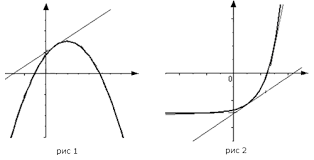
\includegraphics[scale=0.5]{graphics.png}
\caption{Вогнутый и выпуклый графики}
\end{figure}

Продолжаем вспоминать дела давно минувших дней, только уже для конкретных инструментов теорвера. Формулируем
\begin{theorem}[Неравенство Йенсена]
Пусть функция $g(x)$ дифференцируема. Тогда $\forall X$
\begin{enumerate}
    \item $g(x) \cup \Longrightarrow \mathbb{E}g(X) \ge g(\mathbb{E}X)$
    \item $g(x) \cap \Longrightarrow \mathbb{E}g(X) \le g(\mathbb{E}X)$
\end{enumerate}
\end{theorem}

Применяя неравенство Йенсена к нашим баранам, получаем
\begin{theorem}
\begin{enumerate}
    \item $u(x) \cup \Longrightarrow X \succeq \mathbb{E}X$, то есть для такого игрока случайность, заложенная в $X$, предпочтительнее среднего выигрыша. Про таких игроков говорят, что у них \textit{любовь к риску (risk lover)}.
    \item $u(x) \cap \Longrightarrow X \preceq \mathbb{E}X$, то есть такому игроку лучше не играть и довольствоваться стабильностью. Про таких игроков говорят, что у них \textit{отвращение к риску (risk averse)}.
\end{enumerate}
\end{theorem}
Вторая производная неинвариантна по отношению к преобразованию $u(x) \rightarrow au(x) + b$, поэтому часто вводят следующее
\begin{definition}
$R = R(x) = \frac{u''(x)}{u'(x)}$ - коэффициент риска. Очевидно, что $R(x) \ge 0$ - risk lover, $R(x) \le 0$ - risk averse.
\end{definition}

\section{Страхование со стороны клиента}
Пусть клиент страховой фирмы имеет начальный капитал $S$, страдает от случайных потерь $X$ и принял для себя функцию полезности $u(x)$. Пусть фирма требует величину $G$ за полное предотвращение случайных потерь. Тогда должно быть предпочтительнее заплатить $G$, чем потерять $X$, то есть $S - X \preceq S - G$. Можно показать (строчки две, просто определение ф.п. и её неубывание), что, если $\exists G_{max}: \mathbb{E}u(S - X) = u(S - G_{max})$, то клиенту стоит участвовать в страховании $\forall G \le G_{max}$. В зависимости от отношения клиента к риску, выводятся две оценки на $G_{max}$:
\begin{enumerate}
    \item Risk lover: $G_{max} \le \mathbb{E}X$
    \item Risk averse: $G_{max} \ge \mathbb{E}X$
\end{enumerate}

\section{Страхование со стороны страховой компании}
Пусть компания имеет начальный капитал $S_I$, функцию полезности $u_I(x)$ и готова получить с клиента $H$ за полное предотвращение случайных потерь $X$. Соответственно, предпочтение выглядит так: $S_I \preceq S_I - X + H$. Тогда компании стоит участвовать в страховании, если $\exists H_{min}: u_I(S_I) = \mathbb{E}u_I(S_I - X + H_{min})$ и $H \ge H_{min}$. В зависимости от отношения компании к риску, выводятся две оценки на $H_{min}$:
\begin{enumerate}
    \item Risk lover: $H_{min} \le \mathbb{E}X$
    \item Risk averse: $H_{min} \ge \mathbb{E}X$
\end{enumerate}
Объединяя эти результаты с предыдущими, получаем, что страхование возможно только в том случае, если $H_{min} \le G_{max}$ (клиент готов заплатить не больше $G_{max}$, а компания требует не меньше $H_{min}$), а значит можно определить возможность страхования по отношению к риску клиента и компании, учитывая оценки с матожиданием.

\section{Эмпирическое определение функции полезности}
Пусть возникла необходимость определить, какая функция полезности у некоторого игрока, на отрезке $[0, s], s > 0$, если известно, что она строго возрастает. Во-первых, в силу инвариантности $u(x) \sim au(x) + b$, выберем $a, b$ так, чтобы $u(0) = 0, u(s) = 1$. На первом шаге предлагаем клиенту купить лотерейный билет вида $X: \begin{smallmatrix}
0 & s \\
p_1 & 1 - p_1
\end{smallmatrix}$. Пусть клиент готов купить этот билет по цене $x_1 \in [0, s]$. Тогда $u(x_1) = u(0) * p_1 + u(s) * (1 - p_1) = 1 - p_1$. Таким образом, определили значение ф.п. в точке $x_1$. Далее предлагаем ему купить следующие билеты: $X_{21}: \begin{smallmatrix}
0 & x_1 \\
p_{21} & 1 - p_{21}
\end{smallmatrix}$, $X_{22}: \begin{smallmatrix}
x_1 & s \\
p_{22} & 1 - p_{22}
\end{smallmatrix}$, $X_{23}: \begin{smallmatrix}
0 & x_1 & s \\
p_{23} & q_{23} & 1 - p_{23} - q_{23}
\end{smallmatrix}$. В зависимости от цены $x_2$, которую он готов заплатить, например, за третий билет, высчитываем $u(x_2) = \mathbb{E}u(X_{23}) = 1 - p_{23} - p_1q_{23}$. Аналогично для двух других билетов. Продолжая эти шаги, получаем приближение функции полезности с любой степенью точности. Кроме того, достаточно было даже одного шага, но в таком случае его надо было бы повторять с различными вероятностями исходов.

\section{Модель Эрроу}
Модель Эрроу описывает оптимальное поведение клиента страховой компании вне зависимости от функции полезности.

Пусть клиент обладает начальным капиталом $S \ge 0$, функцией полезности $u(x)$ и страдает от случайных потерь $X \ge 0$. За частичное предотвращение потерь клиент готов заплатить $G \in (0, S)$. Страховая компания предлагает частичное возмещение ущерба $I(x)$ (вычет), то есть $0 \le I(X) \le X: \mathbb{E}I(X) = G$. Тем самым потери клиента будут $X - I(X)$ по цене $G$. Клиент готов согласиться на вычет $I^*(x)$, оптимальный с его точки зрения, то есть такой, что $0 \le I^*(X) \le X: \mathbb{E}I^*(X) = G$, а, кроме того, $S - (X - I^*(X)) - G \succeq S - (X - I(X)) - G$, $\forall I(X)$, удовлетворяющей неравенствам выше (вычет клиента с точки зрения клиента даст более предпочтительную ситуацию, чем любой вычет, предлагаемый компанией). Тогда из определения функции полезности получаем модель Эрроу: $$\mathbb{E}u(S - X + I(X) - G) \le \mathbb{E}u(S - X + I^*(X) - G)$$
\begin{theorem}
Пусть $u'(x) \ge 0, u''(x) \le 0$, то есть у клиента отвращение к риску. Тогда оптимальное $I^*(x)$, удовлетворяющее условиям выше, имеет вид $$I^*(x) = \begin{cases}
0, & x \le d^* \\
x - d^*, & x > d^*
\end{cases}$$ для некоторого $d^*$, определённого ниже.
\end{theorem}
\begin{definition}
Значение $d^*$ определяется из условия $\mathbb{E}I^*(X) = G$ и называется \textit{оптимальной франшизой}.
\end{definition}
Заметим, что оптимальный вычет $I^*(x)$ не зависит от начального капитала $S$ и функции полезности $u(x)$. В этом и состоит основная прелесть модели. Дефект же заключается в том, что в условии теоремы нельзя заменить отвращение к риску любовью к нему.

Кроме того, Бенинг приводит способ считать на практике $d^*$, который, ко всему прочему, является следствием похожей и очень полезной формулы для матожидания в случае любой случайной величины (необязательно непрерывной) через функцию распределения. Если есть конечное матожидание случайных потерь (что естественно в жизни), то оптимальная франшиза считается из уравнения $\int_{d^*}^\infty (1 - F(x))dx = G$, где $F(x)$ - функция распределения $X$ (если вдруг кто забыл, $F(x) = \mathbb{P}(X < x)$).

\section{Эмпирические принципы выбора страховых взносов}
Пусть $H$ - величина страхового взноса, который компания требует с клиента. Обозначим функцию распределения возможного ущерба через $F(x)$. Обычно считают, что $H = H(F, \lambda)$, где $\lambda$ - некий параметр, окончательно определяющий величину взноса. Естественно, что, имея лишь выборки потерь клиента, страховая компания будет выбирать взнос по формулам ниже, только меняя матожидание и дисперсию на эмпирические.
\subsection{Принцип оптимального значения(expected value principle)}
$$H = (1 + \lambda)\mathbb{E}X$$
\subsection{Принцип вариации(variance principle)}
$$H = \mathbb{E}X + \lambda\mathbb{D}X$$ Принцип не оч, потому что разные размерности у слагаемых
\subsection{Принцип нулевой полезности(zero utility principle)}
$$\mathbb{E}u_I(S_I + H_{min} - X) = u_I(S_I)$$ $u_I(x)$ - функция полезности страхователя, причём с отвращением к риску ($u_I''(x) \le 0$). Берём $H$, равное $H_{min}$, определённому из уравнения
\subsection{Экспоненциальный принцип(exponential principle)}
Получается из предыдущего выбором $u_I(x) = \frac{1}{\lambda}(1 - e^{-\lambda x})$. $$H = H_{min} = \frac{1}{\lambda}(\mathbb{E}e^{\lambda x})$$
\subsection{Принцип Эшера(Escher principle)} $$H = \frac{\mathbb{E}Xe^{\lambda x}}{\mathbb{E}e^{\lambda x}}$$
\subsection{Суисс-принцип(Swiss principle)} 
(что-то мне подсказывает, что он "швейцарский"). Пусть $f(x) : f'(x) > 0, f''(x) \ge 0$. Тогда $H$ выбирается из уравнения $$\mathbb{E}f(X - \lambda H) = f((1 - \lambda)H), \lambda \in [0, 1]$$
\section{Остальное}
Следующие два раздела, посвящённые индивидуальным и коллективным искам, я намеренно не вношу сюда, поскольку, по-моему, там происходит исключительно подсчёт частных случаев и различных моментов для вводимых с.в. Оказалось, что он может спросить и по ним, но вопрос звучит одинаково: "Сформулируйте какую-нибудь теорему про случайные суммы". Поэтому вот парочка теорем на выбор:
\begin{definition}
Пусть $X_i$ - величина страховой выплаты $i$-му клиенту, а $N$ - неотрицательная целочисленная случайная величина, принимающая значение $i = 0, 1, \ldots$ с вероятностью $p_i$. Тогда величина общих выплат $X = (X_1 + \ldots + X_N)\mathbb{1}_{[1, +\infty]}(N)$ называется \textit{случайной суммой}. Мы везде предполагаем, что $N, X_1, \ldots$ - независимые случайные величины, а $X_1, X_2, \ldots$ - одинаково распределённые случайные величины.
\end{definition}
\begin{theorem}
В обозначениях выше верны равенства $$\ME X = \ME X_1 \cdot \ME N,$$ $$\D X = \ME N \cdot \D X_1 + (\ME X_1)^2 \cdot \D N.$$
\end{theorem}
\begin{theorem}
Справедливы формулы: $$F_X(x) = \mathbb{1}_{(0, +\infty)}\prob(N = 0) + \sum\limits_{k = 1}^{+\infty}\prob(X_1 + \ldots + X_k < x)\prob(N = k),$$ $$\chi_X(t) = g_N(\chi_{X_1}(t)),$$ где $F_X(x)$ - функция распределения, $\chi_X(t)$ - характеристическая функция случайной величины $X$, $g_N(s) = \ME s^N$ - производящая функция.
\end{theorem}
\newpage
\section{Заметки об экзамене}
Главная проблема всего курса - найти Бенинга, когда вы хотите что-нибудь ему сдать. Ходить на пары очень необязательно, хотя очень просто на них получить автомат: достаточно решить несколько задач из тех, что он даст. Задачи несложные, но потом вы встречаетесь с проблемой, описанной выше. 

Аналогичная проблема есть с досроком. Он ставит его тогда, когда захочет, и ооочень хочет поскорее свалить. Например, у нас досрок был параллельно с зачётом по лингве, и те, кто сдал зачёт чуть позже, застали закрытую на ключ дверь и ушедшего Бенинга. На досроке он спрашивал исключительно по первым пяти главам.

Что же касается экзамена, то чем позже заходил человек, тем более поздние главы он спрашивал. В конце начал у людей спрашивать про теоремы о случайных суммах. А обычно любит спросить детерминированный эквивалент, модель Эрроу и что-нибудь из парадоксов. Оценки ниже 4 на экзамене нет. Либо ты отвечаешь и получаешь 5, либо не отвечаешь и получаешь 4. По-видимому, на эту 4 вы нарабатываете, пока пишете билет. Правда, вы его пишете дома и на свой выбор пару теорем, но формально билет есть (да-да, лучшая кафедра).
\end{document}
